\begin{frame}
  \frametitle{What Prevents Perfection}
  \framesubtitle{Are We Stuck Here?}
  \begin{itemize}
    \item  People are the Common Factor

          \note[item]<1-> {\scriptsize{Within every domain of Cybersecurity people play a key and decisive role for ensuring success or failure. \textcite{bacchiWhyStudyProblematizations2012} suggests that within any policy discussion, the proposal itself is a ``prescriptive text'' that frames and represents an underlying problem in a particular way. Policy is how we constitute the problem. In cybersecurity people appear in several places within the framing of the problem: as the attackers seeking to subvert the controls and protections; as those attempting to prevent attacks by implementing countermeasures and security policies; as those who may inadvertently empower attacks by violating policy or subverting countermeasures; and as intentional internal bad actors. People are a common factor. As this illustration from (Bracchi, 2012) suggests.  }}

 \item[] 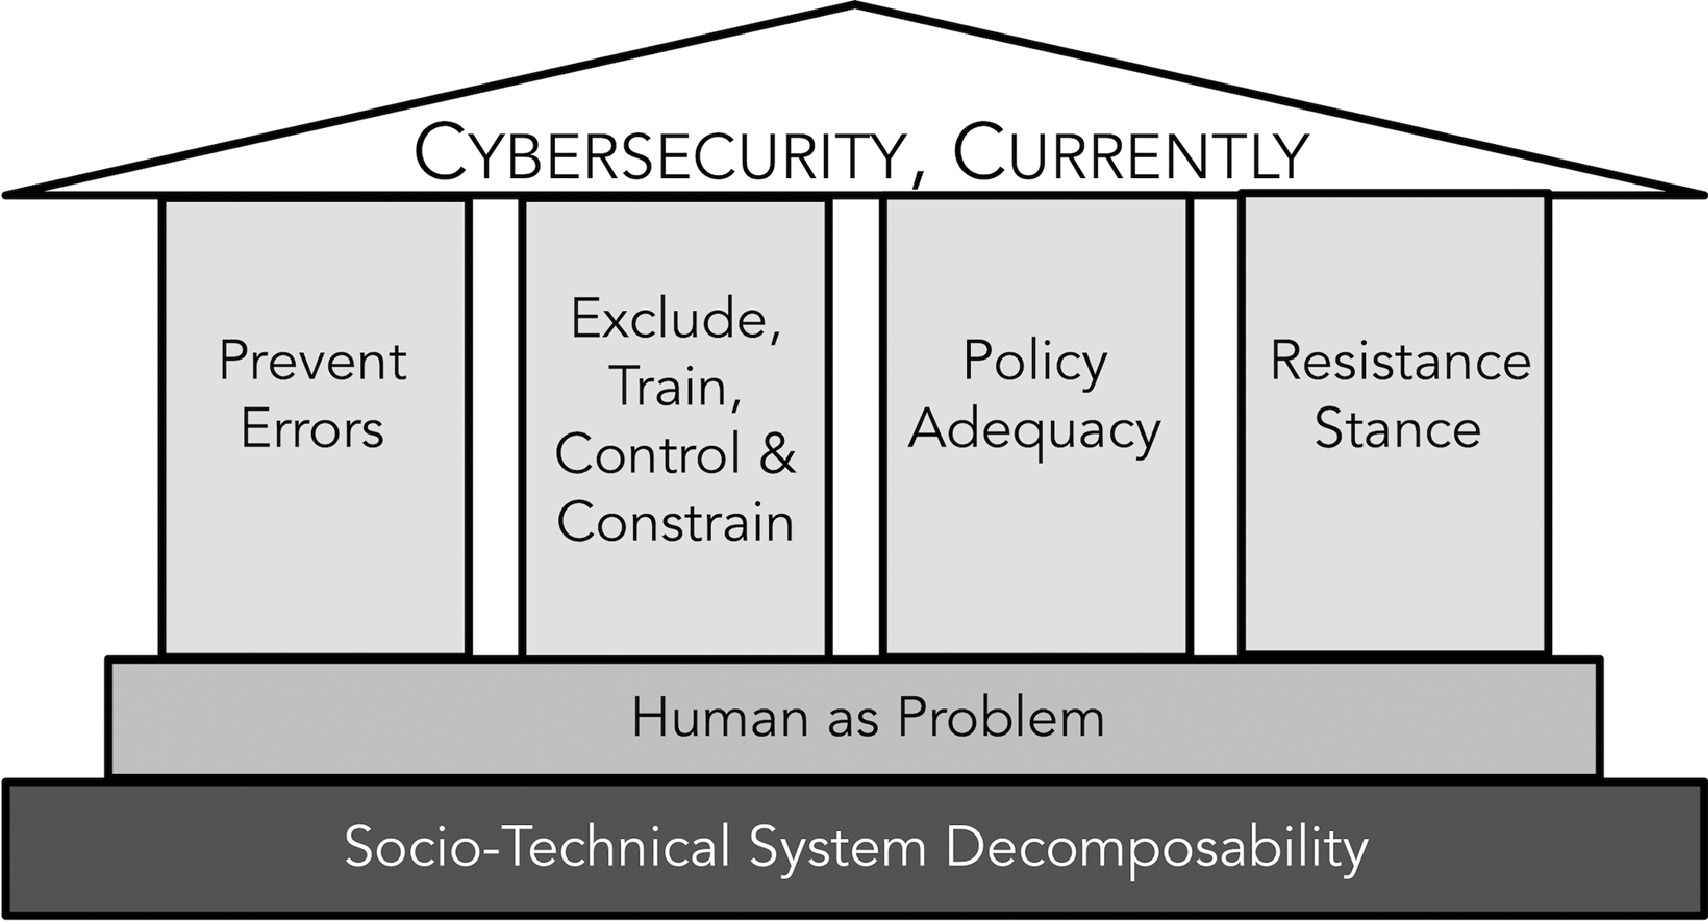
\includegraphics[width=0.65\textwidth]{humanproblem}

    \item<2-> Are People the Common Solution?
          \note[item]<2-> {\scriptsize{As nearly, if not all, issues in cybersecurity involve human actors in various roles; it follows that human actors are the most plausible solution to addressing cybersecurity problems \parencite{zimmermannMovingHumanasproblemHumanassolution2019}.}}


    \item<3-> People in the plural, not Person in the Singular
          \note[item]<3->{\scriptsize{Historically, individual mistakes, laziness, apathy, ignorance, and other characteristics best collectively addressed as moral judgements have been considered the underlying cause of cybersecurity failure. Very few studies focused on broader questions of human behavior generally or the social psychology of cybersecurity \parencite{renaudContemplatingHumancentredSecurity2017}.}}

    \item<4-> The Problem may not be People, but Perception

          \note[item]<4->{\scriptsize{If we understand people as external entities who have to work both with and within the environment, then our approach to cybersecurity must change, and with it the resulting outcomes. If we perceive individual failures as the underlying cause of cybersecurity failure, we can't examine the possibility that our problem definition is structured poorly. What if the problem isn't individual training, apathy, competence, and so forth, but social attitudes and perceptions?}}


  \end{itemize}
\end{frame}
